\documentclass[conference]{IEEEtran}
\IEEEoverridecommandlockouts
% The preceding line is only needed to identify funding in the first footnote. If that is unneeded, please comment it out.
\usepackage{cite}
\usepackage{amsmath,amssymb,amsfonts}
\usepackage{algorithmic}
\usepackage{graphicx}
\usepackage{textcomp}
\usepackage{tikz}
\usetikzlibrary{positioning,arrows.meta}
\usepackage{xcolor}
\def\BibTeX{{\rm B\kern-.05em{\sc i\kern-.025em b}\kern-.08em
    T\kern-.1667em\lower.7ex\hbox{E}\kern-.125emX}}
\begin{document}

\title{Análise da Influência de Subconjuntos de Características Biológicas na Predição do Risco de Extinção de Espécies por Aprendizado de Máquina}

\author{\IEEEauthorblockN{Danniel Vieira Holanda}
\IEEEauthorblockA{\textit{Engenharia da Computação} \\
\textit{CEFET-MG Campus V.}\\
Divinópolis, Brasil \\
dannielvh7@gmail.com}
}

\maketitle

%\begin{abstract}
%This document is a model and instructions for \LaTeX.
%This and the IEEEtran.cls file define the components of your paper [title, text, heads, etc.]. *CRITICAL: Do Not Use Symbols, Special Characters, Footnotes, 
%or Math in Paper Title or Abstract.
%\end{abstract}

%\begin{IEEEkeywords}
%component, formatting, style, styling, insert
%\end{IEEEkeywords}

\section{Introdução}

A perda de biodiversidade é um dos principais desafios ambientais da atualidade. As atividades humanas vêm provocando alterações profundas nos ecossistemas e aumentando a vulnerabilidade de diversas espécies, o que torna necessária a adoção de estratégias eficientes de conservação \cite{b1}. Nesse cenário, a identificação de espécies ameaçadas e a compreensão dos fatores associados ao risco de extinção são fundamentais para direcionar ações prioritárias. Para isso, a Lista Vermelha da União Internacional para a Conservação da Natureza (IUCN) se destaca como uma das principais ferramentas utilizadas para a avaliação do estado de conservação das espécies \cite{b2}.

O avanço na disponibilidade de dados biológicos e ecológicos tem possibilitado o uso de técnicas computacionais no suporte a esses estudos. Algoritmos de Aprendizado de Máquina conseguem analisar grandes volumes de dados e identificar padrões de risco que complementam as abordagens tradicionais de avaliação \cite{b3}. Entre os atributos analisados, características biológicas como massa corporal, fecundidade, tempo de geração, capacidade de dispersão e especificidade de habitat podem estar diretamente relacionadas à vulnerabilidade das espécies.

Estudos anteriores têm investigado a relação entre características biológicas e o risco de extinção. Uma revisão sobre essa relação observou que a importância das características pode variar entre diferentes grupos taxonômicos \cite{b4}. Posteriormente, foi realizada uma análise sobre a capacidade de diferentes características em predizer o risco de extinção em grupos terrestres, identificando que algumas apresentam padrões mais consistentes, enquanto outras possuem relevância dependente do grupo analisado \cite{b5}.

Apesar desses avanços, ainda existem desafios relacionados à seleção das características utilizadas em modelos preditivos. Não está completamente estabelecido como a quantidade e as diferentes combinações de variáveis influenciam o desempenho dos modelos de Aprendizado de Máquina, especialmente quando diferentes grupos taxonômicos são comparados. Dessa forma, torna-se relevante investigar se subconjuntos reduzidos de características podem apresentar desempenho semelhante ou superior à utilização de um conjunto maior de variáveis.

Diante desse cenário, o objetivo deste trabalho é avaliar o impacto de diferentes subconjuntos de características biológicas na predição do risco de extinção via Aprendizado de Máquina. A pesquisa utiliza dados públicos sobre mamíferos e aves, testando combinações variadas de atributos para medir como a escolha e o número de variáveis influenciam a precisão dos modelos, além de verificar se os padrões observados se mantêm entre ambos os grupos.

\section{Revisão da Literatura}

A utilização de características biológicas para predizer o risco de extinção permite complementar as avaliações tradicionais de conservação. Atributos como tamanho corporal, fecundidade, tempo de geração, capacidade de dispersão e especificidade de habitat podem estar associados à vulnerabilidade das espécies. Entretanto, essas relações variam entre grupos taxonômicos, tornando relevante investigar quais características contribuem para a predição do risco \cite{b4,b5}.

Chichorro \textit{et al.} \cite{b5} investigaram a relação entre características biológicas e risco de extinção em diferentes grupos de organismos terrestres, utilizando dez potenciais preditores. Os resultados indicaram que a especificidade de habitat e características associadas a histórias de vida mais lentas apresentaram relações relevantes em diversos grupos, enquanto outros atributos tiveram importância mais restrita a determinados grupos taxonômicos. Embora o estudo tenha identificado padrões gerais e específicos, seu foco não foi avaliar diretamente como a quantidade e a composição dos atributos afetam o desempenho preditivo de modelos de Aprendizado de Máquina.

Nesse contexto, Zizka \textit{et al.} \cite{b6} desenvolveram o IUCNN, uma abordagem baseada em redes neurais profundas para aproximar categorias de risco da Lista Vermelha da IUCN utilizando dados públicos, especialmente registros de ocorrência geográfica. Os autores demonstraram o potencial de modelos computacionais para auxiliar na avaliação de espécies, diante das limitações de cobertura taxonômica e geográfica das avaliações existentes. Entretanto, a abordagem difere da presente pesquisa por utilizar dados de ocorrência e aprendizagem profunda, enquanto este trabalho investiga a influência de subconjuntos de características biológicas sobre o desempenho da classificação.

Branco, Correia e Cardoso \cite{b7} realizaram uma revisão sistemática sobre a aplicação de Aprendizado de Máquina em problemas relacionados às ameaças às espécies e à conservação. Os autores identificaram o emprego crescente de técnicas como modelos bayesianos, métodos de conjunto e algoritmos baseados em árvores, ressaltando que a escolha do método depende da natureza dos dados e do problema estudado. A revisão também destaca a importância da interpretabilidade, especialmente em aplicações nas quais compreender os fatores associados às previsões pode auxiliar decisões de conservação. Nesse sentido, investigar modelos que mantenham desempenho satisfatório com menos atributos pode contribuir para análises mais simples e para aplicações em cenários com informações biológicas limitadas.

Outros estudos aplicaram Aprendizado de Máquina a grupos específicos. Loiseau \textit{et al.} \cite{b8} utilizaram informações de ocorrência, características biológicas, taxonomia e utilização humana para predizer o estado de conservação de peixes marinhos, identificando possíveis diferenças em relação às classificações existentes na Lista Vermelha. Entretanto, a combinação de diferentes fontes de informação dificulta isolar a contribuição das características biológicas. De maneira semelhante, Pacifici \textit{et al.} \cite{b9} utilizaram Random Forest para investigar o risco de extinção de primatas neotropicais, observando a relevância de fatores ambientais e de pressões humanas, como fragmentação de habitat e caça.

Van Zuijlen \textit{et al.} \cite{b10}, por sua vez, investigaram o risco de extinção de briófitas europeias por meio de modelos de Random Forest que combinavam variáveis bioclimáticas e características biológicas. Os resultados destacaram a contribuição dos fatores climáticos, embora atributos biológicos também apresentassem relevância. Em conjunto, esses estudos demonstram que a capacidade preditiva das variáveis depende do organismo analisado e dos fatores considerados, o que dificulta estabelecer um conjunto universal de atributos para diferentes grupos taxonômicos \cite{b5,b9,b10}.

Apesar dos avanços apresentados, permanece relevante investigar sistematicamente como a quantidade e a composição das características biológicas influenciam o desempenho preditivo. Enquanto estudos anteriores priorizam a identificação de fatores associados ao risco ou combinam diferentes fontes de informação, a avaliação de quantos atributos são necessários para preservar o desempenho dos modelos constitui uma questão complementar. Essa análise também permite verificar se os subconjuntos mais adequados variam entre grupos taxonômicos.

A presente pesquisa busca contribuir para essa lacuna utilizando a base de dados de Chichorro \textit{et al.} \cite{b5}, com foco em mamíferos e aves. Serão comparados modelos de Aprendizado de Máquina treinados com diferentes subconjuntos de características biológicas, avaliando-se a relação entre a quantidade de atributos e o desempenho preditivo. A comparação entre os grupos permitirá investigar se a redução de variáveis produz efeitos semelhantes ou se as características mais relevantes diferem entre mamíferos e aves. Assim, o estudo desloca o foco da identificação de atributos associados ao risco para a avaliação de quais e quantas características são necessárias para obter modelos preditivos eficientes.

\section{Materiais e Métodos}

\subsection{Base de Dados}

Este estudo utiliza a base de dados associada ao trabalho de Chichorro et al. \cite{b5}, intitulada ``Trait-based prediction of extinction risk across terrestrial taxa''. O conjunto reúne informações sobre características biológicas de espécies e seus respectivos níveis de risco de extinção. A pesquisa concentra-se nos registros de mamíferos e aves disponíveis na base, utilizando as características biológicas como variáveis preditoras e o risco de extinção como variável-alvo.

Entre os atributos investigados no estudo original estão características relacionadas ao tamanho corporal, à fecundidade, ao tempo de geração, à capacidade de dispersão e à especificidade de habitat. A seleção definitiva das variáveis dependerá da estrutura dos arquivos utilizados e da disponibilidade de informações para os dois grupos taxonômicos.

Inicialmente, será realizada uma análise exploratória para identificar a quantidade de registros, o número de atributos, os tipos de variáveis, a distribuição das classes e a ocorrência de valores ausentes ou duplicados. Esses dados serão utilizados para caracterizar a base antes e após o pré-processamento, permitindo documentar a quantidade de instâncias efetivamente utilizada nos experimentos.

\subsection{Pré-processamento}

Os registros serão separados por grupo taxonômico, mantendo-se apenas as informações necessárias à modelagem. A variável-alvo será definida a partir das categorias de risco de extinção presentes na base. Como estratégia inicial, será considerada uma classificação binária entre espécies de menor preocupação (LC e NT) e espécies ameaçadas (VU, EN e CR). Essa agregação será aplicada somente após confirmar a presença e a consistência dessas categorias. Registros sem avaliação ou com dados insuficientes não serão classificados automaticamente como espécies de baixo risco.

Os valores ausentes serão identificados e tratados de acordo com a quantidade e o tipo de informação disponível. Quando necessário, poderão ser utilizadas a mediana para variáveis numéricas e a categoria mais frequente para variáveis categóricas. Atributos não informativos para a predição, como identificadores de espécies, serão excluídos das entradas dos modelos. Variáveis categóricas serão codificadas numericamente e, quando necessário, as variáveis numéricas serão padronizadas.

Para evitar vazamento de dados, os parâmetros de imputação, codificação e padronização serão ajustados exclusivamente nos dados de treinamento de cada experimento. A distribuição das classes também será examinada para identificar possíveis desbalanceamentos e determinar a necessidade de estratégias de ponderação durante o treinamento.

\subsection{Modelos de Aprendizado de Máquina}

O problema será tratado como uma tarefa de classificação supervisionada. Serão avaliados inicialmente dois algoritmos: Regressão Logística e Random Forest. A Regressão Logística será utilizada como modelo de referência devido à sua simplicidade e interpretabilidade. A Random Forest combina árvores de decisão e permite representar relações não lineares entre as características biológicas, oferecendo uma abordagem complementar para a tarefa de classificação \cite{b11,b12}.

A comparação entre os algoritmos será realizada utilizando os mesmos conjuntos de dados e protocolos de avaliação. O experimento inicial utilizará todas as características elegíveis. Em seguida, serão avaliados subconjuntos menores, variando a quantidade e a composição dos atributos. Quando o número de variáveis permitir, serão testadas todas as combinações possíveis para cada tamanho de subconjunto.

A seleção dos atributos será realizada apenas nos dados de treinamento, com o objetivo de identificar quais subconjuntos preservam melhor o desempenho preditivo. Dessa forma, será possível investigar se a redução de variáveis mantém resultados próximos aos obtidos com o conjunto completo e se essa relação difere entre mamíferos e aves.

\subsection{Protocolo Experimental e Métricas}

Os experimentos serão conduzidos separadamente para mamíferos e aves. Uma análise conjunta poderá ser realizada para complementar a comparação, desde que a composição dos dados permita uma avaliação adequada. Em cada experimento, os dados serão divididos em conjuntos de treinamento (80\%) e teste (20\%), com estratificação pela variável-alvo e utilização de uma semente aleatória fixa.

O conjunto de treinamento será utilizado para ajustar os modelos e realizar validação cruzada estratificada de cinco partições. A seleção dos subconjuntos de características e eventuais ajustes de hiperparâmetros ocorrerão nessa etapa. Após a definição das configurações, os modelos serão treinados com os dados de treinamento e avaliados no conjunto de teste, mantido isolado durante as decisões metodológicas.

O desempenho será avaliado por meio de acurácia, precisão, revocação (recall) e F1-score. A acurácia mede a proporção de classificações corretas; a precisão indica a proporção de previsões positivas corretas; a revocação mede a proporção de espécies da classe positiva identificadas pelo modelo; e o F1-score representa a média harmônica entre precisão e revocação. A classe de maior risco de extinção será considerada positiva, permitindo observar a capacidade dos modelos de identificar espécies ameaçadas. A matriz de confusão também será utilizada para examinar os erros de classificação.

Os resultados serão comparados considerando o número de atributos, a composição dos subconjuntos e o algoritmo utilizado. Serão registrados o desempenho médio observado na validação cruzada e as métricas obtidas no teste final. A análise buscará identificar combinações que reduzam a quantidade de características sem comprometer significativamente o desempenho, além de verificar possíveis diferenças entre os grupos taxonômicos.

\subsection{Fluxo Metodológico}

A Figura~\ref{fig:fluxo_metodologico} resume as principais etapas da pesquisa.

\begin{figure}[htbp]
\centering
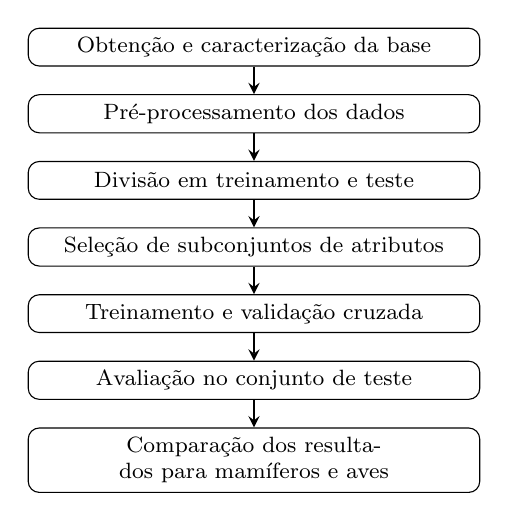
\begin{tikzpicture}[
    node distance=0.35cm,
    etapa/.style={
        rectangle,
        rounded corners,
        draw=black,
        align=center,
        text width=5.5cm,
        minimum height=0.48cm,
        font=\footnotesize
    },
    seta/.style={->, thick, >=stealth}
]
\node[etapa] (dados) {Obtenção e caracterização da base};
\node[etapa, below=of dados] (pre) {Pré-processamento dos dados};
\node[etapa, below=of pre] (div) {Divisão em treinamento e teste};
\node[etapa, below=of div] (sub) {Seleção de subconjuntos de atributos};
\node[etapa, below=of sub] (modelos) {Treinamento e validação cruzada};
\node[etapa, below=of modelos] (teste) {Avaliação no conjunto de teste};
\node[etapa, below=of teste] (analise) {Comparação dos resultados para mamíferos e aves};

\draw[seta] (dados) -- (pre);
\draw[seta] (pre) -- (div);
\draw[seta] (div) -- (sub);
\draw[seta] (sub) -- (modelos);
\draw[seta] (modelos) -- (teste);
\draw[seta] (teste) -- (analise);
\end{tikzpicture}
\caption{Fluxo metodológico da pesquisa.}
\label{fig:fluxo_metodologico}
\end{figure}

O fluxo metodológico organiza as etapas necessárias para avaliar a influência da quantidade e da composição das características biológicas na predição do risco de extinção. Inicialmente, a base de dados será caracterizada e pré-processada; em seguida, os dados serão divididos em conjuntos de treinamento e teste. Diferentes subconjuntos de atributos serão utilizados no treinamento e na validação dos modelos de Regressão Logística e Random Forest, permitindo comparar seus desempenhos com base nas métricas definidas. Por fim, os resultados serão analisados separadamente para mamíferos e aves, buscando identificar se a redução de atributos preserva a capacidade preditiva e se os efeitos observados diferem entre os grupos taxonômicos.

%\section{Ease of Use}

%\section*{Acknowledgment}


\begin{thebibliography}{00}

\bibitem{b1}
IPBES, \textit{Global Assessment Report on Biodiversity and Ecosystem Services of the Intergovernmental Science-Policy Platform on Biodiversity and Ecosystem Services}. Bonn, Germany: IPBES Secretariat, 2019.

\bibitem{b2}
IUCN, \textit{IUCN Red List Categories and Criteria: Version 3.1}, 2nd ed. Gland, Switzerland and Cambridge, U.K.: International Union for Conservation of Nature, 2012.

\bibitem{b3}
M. Di Marco \textit{et al.}, ``Drivers of extinction risk in African mammals: The interplay of distribution state, human pressure, conservation response and species biology,'' \textit{Proceedings of the Royal Society B: Biological Sciences}, vol. 281, 2014.

\bibitem{b4}
F. Chichorro, A. Juslén, and P. Cardoso, ``A review of the relation between species traits and extinction risk,'' \textit{Biological Conservation}, vol. 237, pp. 220--229, 2019.

\bibitem{b5}
F. Chichorro \textit{et al.}, ``Trait-based prediction of extinction risk across terrestrial taxa,'' \textit{Biological Conservation}, vol. 274, Art. no. 109738, 2022.

\bibitem{b6} D. Zizka, M. Silvestro, F. Andermann, S. Ficetola, and M. Pellissier, ``IUCNN -- Deep learning approaches to approximate species' extinction risk,'' \textit{Diversity and Distributions}, vol. 28, pp. 114--127, 2022, doi: 10.1111/ddi.13450.

\bibitem{b7} V. V. Branco, L. Correia, and P. Cardoso, ``The use of machine learning in species threats and conservation analysis,'' \textit{Biological Conservation}, vol. 283, Art. no. 110091, 2023, doi: 10.1016/j.biocon.2023.110091.

\bibitem{b8} L. Loiseau et al., ``Inferring the extinction risk of marine fish to inform global conservation priorities,'' \textit{Diversity and Distributions}, 2024, doi: 10.1111/ddi.13961.

\bibitem{b9} M. Pacifici, C. Rondinini, and L. Santini et al., ``Synergistic effects of habitat fragmentation and hunting on the extinction risk of neotropical primates,'' \textit{Biodiversity and Conservation}, vol. 32, pp. 2847--2866, 2023, doi: 10.1007/s10531-023-02623-w.

\bibitem{b10} A. Van Zuijlen et al., ``Extinction risk of European bryophytes predicted by bioclimate and traits,'' \textit{Biological Conservation}, vol. 293, Art. no. 110593, 2024.

\bibitem{b11}
L. Breiman, ``Random forests,''
Machine Learning, vol. 45, pp. 5--32, 2001,
doi: 10.1023/A:1010933404324.

\bibitem{b12}
F. Pedregosa et al., ``Scikit-learn: Machine learning in Python,''
Journal of Machine Learning Research, vol. 12, pp. 2825--2830, 2011.

\end{thebibliography}

\end{document}
